\subsection{Steel beams}

\begin{figure}
  \begin{center}
  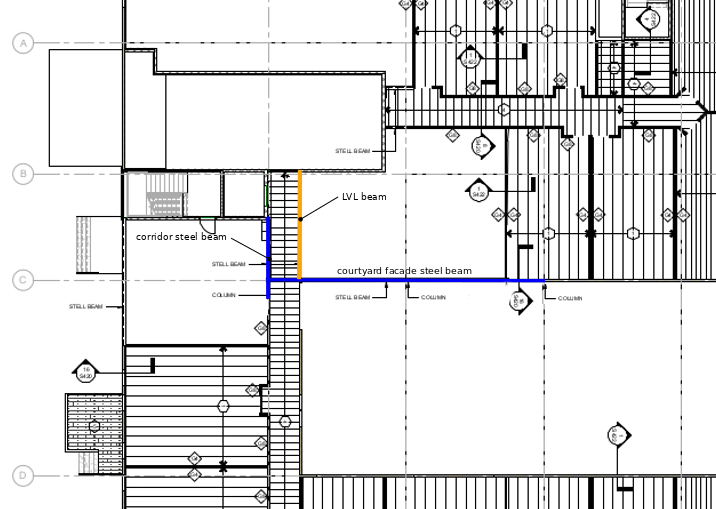
\includegraphics[width=120mm]{figures/steel_beams_key_plan}
  \end{center}
  \caption{Second floor beams key plan.}\label{fg_2nd_floor_beams_key_plan}
\end{figure}

\subsubsection{Steel beam at courtyard facade}
Continuous beam supporting the second floor trusses between the axes 1, 2 and 3 (see figure \ref{fg_2nd_floor_beams_key_plan}). The beam has two equal spans; L= 8.31 m ($27' - 3''$).

\paragraph{Design loads.}
The design loads are show in table \ref{tb_CD_reactions}. The beam then carries a load of $19.785\ kN$ each $0.6 m (24'')$. 

\begin{table}
  \begin{center}
  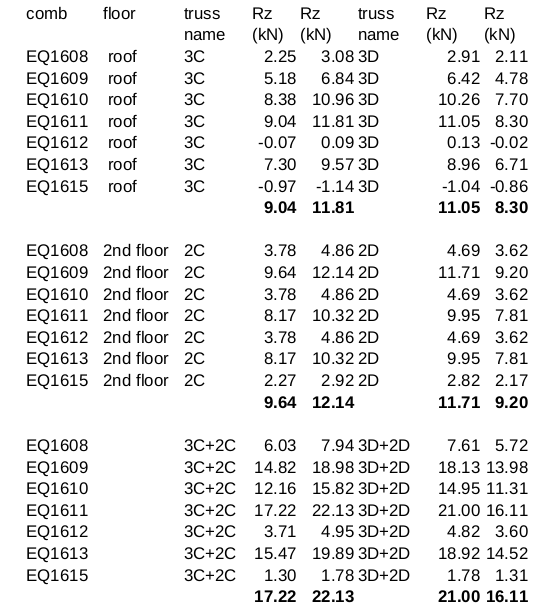
\includegraphics[width=75mm]{figures/CD_reactions}
  \end{center}
  \caption{Steel beam at courtyard facade.Trusses reactions.}\label{tb_CD_reactions}
\end{table}

\paragraph{Structural design of the beam.}

\subparagraph{Loads.}

\begin{equation}
  w_{load}= 19.785\ kN/m
\end{equation}

\subparagraph{Internal forces on each structural channel.}

\noindent Maximum induced moment:

\begin{equation}
  M_{max}= 170.61\ kN m
\end{equation}

\noindent Maximum induced shear:

\begin{equation}
  V_{max}= 102.71\ kN
\end{equation}

\subparagraph{Structural channel (C380X50.4) mechanical properties.}
Steel: ASTM A-572

\noindent Shear strength:
\begin{equation}
  V_u= 463.52\ kN 
\end{equation}
\noindent Structural shear check: $V_u = 463.52 > 102.71 = V_{max} \implies OK$

\noindent Resisting moment:
\begin{equation}
  M_u= 171.88\ kN\cdot m
\end{equation}

\noindent Structural bending check: $M_U = 171.88 > 170.61 = M_{max} \implies OK$

\subparagraph{Bending stiffness.}
The deflection obtained is:

\begin{equation}
  \Delta_{TL}= 18.72\ mm= \frac{span}{444} < \frac{L}{360} \implies OK
\end{equation}

\subsubsection{Steel beam at corridor}
This beam supports the second floor trusses near the elevator well (see figure \ref{fg_2nd_floor_beams_key_plan}) . It has a main span of 3.97 m long ($13' - 5/16''$)  and a cantilever that spans 1.04 m ($3'-4''$).

\paragraph{Design loads.}
The design loads are show in table \ref{tb_E_reactions}. The beam then carries a load of $31.66\ kN$ each $0.6 m (24'')$. 

\begin{table}
  \begin{center}
  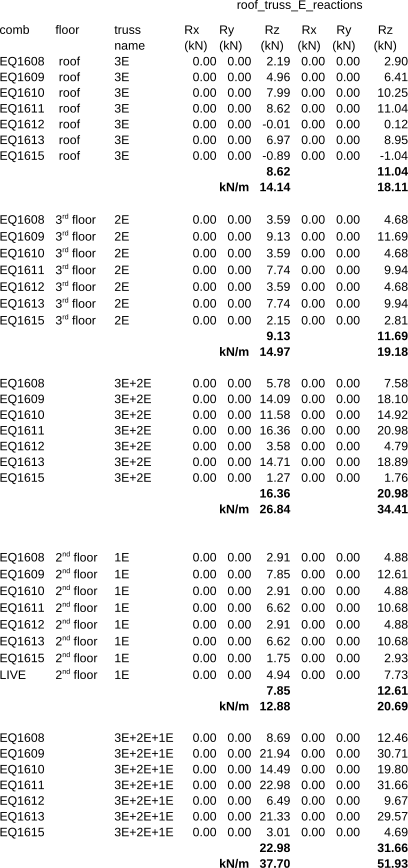
\includegraphics[width=75mm]{figures/E_reactions}
  \end{center}
  \caption{Steel beam at corridor. Trusses reactions.}\label{tb_E_reactions}
\end{table}

\paragraph{Structural design of the beam.}

\subparagraph{Loads.}

\begin{equation}
  w_{load}= 51.94\ kN/m
\end{equation}

\subparagraph{Internal forces on each structural channel.}

\noindent Maximum induced moment:

\begin{equation}
  M_{max}= 147.94\ kN m
\end{equation}

\noindent Maximum induced shear:

\begin{equation}
  V_{max}= 140.13\ kN
\end{equation}

\subparagraph{Structural shape (W14X30) mechanical properties.}
Steel: ASTM A-572

\noindent Shear strength:
\begin{equation}
  V_u= 254.63\ kN 
\end{equation}
\noindent Structural shear check: $V_u = 254.63 > 140.13 = V_{max} \implies OK$

\noindent Resisting moment:
\begin{equation}
  M_u= 160.10\ kN\cdot m
\end{equation}

\noindent Structural bending check: $M_U = 160.10 > 147.94 = M_{max} \implies OK$

\subparagraph{Bending stiffness.}
The deflection obtained is:

\begin{equation}
  \Delta_{TL}=9.04\ mm= \frac{L}{439} < \frac{span}{360} \implies OK
\end{equation}
